\documentclass{article}
\usepackage[margin=1in]{geometry}
\usepackage{graphicx}
\usepackage[dvipsnames,table]{xcolor}
\usepackage[utf8]{inputenc}
\usepackage{siunitx}
\usepackage[american,siunitx]{circuitikz}
\usepackage{amsmath}
\usepackage{svg}
\usepackage{booktabs}
\usepackage{float}
\usepackage{xparse, xfp}
\usepackage{multirow}
\usepackage{tikz}
\usepackage{karnaugh-map}
\usepackage{pdfpages}
\usepackage{pdflscape}
\usepackage{hyperref}
\usepackage{adjustbox}
\usepackage[T1]{fontenc}
\usepackage{beramono}% monospaced font with bold variant
\usepackage{listings}
\lstdefinelanguage{VHDL}{  morekeywords={library,use,all,entity,is,port,in,out,end,architecture,of,    begin,and  ,LIBRARY,USE,ALL,ENTITY,IS,PORT,IN,OUT,END,ARCHITECTURE,OF,    BEGIN,AND},  morecomment=[l]--}
\usepackage{xcolor}
\colorlet{keyword}{blue!100!black!80}
\colorlet{comment}{green!90!black!90}
\lstdefinestyle{vhdl}{  language     = VHDL,  basicstyle   = \ttfamily,  keywordstyle = \color{keyword}\bfseries,  commentstyle = \color{comment}}


\newcommand{\overbar}[1]{\mkern 1.5mu\overline{\mkern-1.5mu#1\mkern-1.5mu}\mkern 1.5mu}
\hypersetup{
    colorlinks=true,
    linkcolor=blue,
    filecolor=magenta,      
    urlcolor=cyan,
}
\usepackage{caption} 

\makeatletter
\ctikzset{lx/.code args={#1 and #2}{ 
  \pgfkeys{/tikz/circuitikz/bipole/label/name=\parbox{1cm}{\centering #1  \\ #2}}
    \ctikzsetvalof{bipole/label/unit}{}
    \ifpgf@circ@siunitx 
        \pgf@circ@handleSI{#2}
        \ifpgf@circ@siunitx@res 
            \edef\pgf@temp{\pgf@circ@handleSI@val}
            \pgfkeyslet{/tikz/circuitikz/bipole/label/name}{\pgf@temp}
            \edef\pgf@temp{\pgf@circ@handleSI@unit}
            \pgfkeyslet{/tikz/circuitikz/bipole/label/unit}{\pgf@temp}
        \else
        \fi
    \else
    \fi
}}

\ctikzset{lx^/.style args={#1 and #2}{ 
    lx=#2 and #1,
    \circuitikzbasekey/bipole/label/position=90 } 
}

\ctikzset{lx_/.style args={#1 and #2}{ 
    lx=#1 and #2,
    \circuitikzbasekey/bipole/label/position=-90 } 
}
\makeatother

\captionsetup[table]{skip=10pt}

\usetikzlibrary{calc, automata, positioning}
%\usepackage[landscape]{geometry}
\renewcommand{\thesubsection}{\thesection.\alph{subsection}}
\newcommand{\equal}{=}
\newcommand{\greyrule}{\arrayrulecolor{black!30}\midrule\arrayrulecolor{black}}
\makeatletter
\newcommand\currcoor{\the\tikz@lastxsaved,\the\tikz@lastysaved}
\makeatother
\newcolumntype{:}{@{\hskip\tabcolsep\color{black!30}\vrule\hskip\tabcolsep}}

\ExplSyntaxOn
\NewExpandableDocumentCommand \groupify { O{\,\allowbreak} m m }
  { \jakob_groupify:nnn {#1} {#2} {#3} }
\cs_new:Npn \jakob_groupify:nnn #1 #2 #3
  { \__jakob_groupify_loop:nnw { 1 } {#2} #3 \q_recursion_tail {#1} \q_recursion_stop }
\cs_new:Npn \__jakob_groupify_loop:nnw #1 #2 #3
  {
    \quark_if_recursion_tail_stop:n {#3}
    \exp_not:n {#3}
    \int_compare:nNnTF {#1} = {#2}
      { \__jakob_groupify_sep:n }
      { \exp_args:Nf \__jakob_groupify_loop:nnw { \int_eval:n { #1+1 } } }
          {#2}
  }
\cs_new:Npn \__jakob_groupify_sep:n #1 #2 \q_recursion_tail #3
  {
    \tl_if_empty:nF {#2} { \exp_not:n {#3} }
    \__jakob_groupify_loop:nnw { 1 } {#1}
    #2 \q_recursion_tail {#3}
  }
\ExplSyntaxOff

\title{ECE 4300\\Discrete System Design Using VHDL\\\,\\Midterm 1}
 \author{Choi Tim Antony Yung (ID:013499993)}
\begin{document}
 \maketitle

% \thispagestyle{empty}
% \setcounter{page}{0}
 \newpage

\pagenumbering{gobble}

\section{Combinational Circuit}

\subsection*{Code}
\subsubsection*{D Flip-flop}
\lstinputlisting[style=VHDL]{ECE4304_Midterm1_VHDL/ECE4304_Midterm1_VHDL.srcs/sources_1/new/DFlipflop.vhd}
\;\\
\subsubsection*{Combinational Circuit}
\lstinputlisting[style=VHDL]{ECE4304_Midterm1_VHDL/ECE4304_Midterm1_VHDL.srcs/sources_1/new/ECE4304_Midterm1_1.vhd}
\;\\
\subsubsection*{Testbench}
\lstinputlisting[style=VHDL]{ECE4304_Midterm1_VHDL/ECE4304_Midterm1_VHDL.srcs/sim_1/new/ECE4304_Midterm1_1_tb.vhd}
\;\\
\subsection*{Simulation Result}
As can be seen in figure \ref{fig:1}, all possible input combination was simulated and the circuit behave as expected with no mismatch found.
\begin{figure}[H]
  \centering
  \caption{Simulation Waveform of the Circuit}
  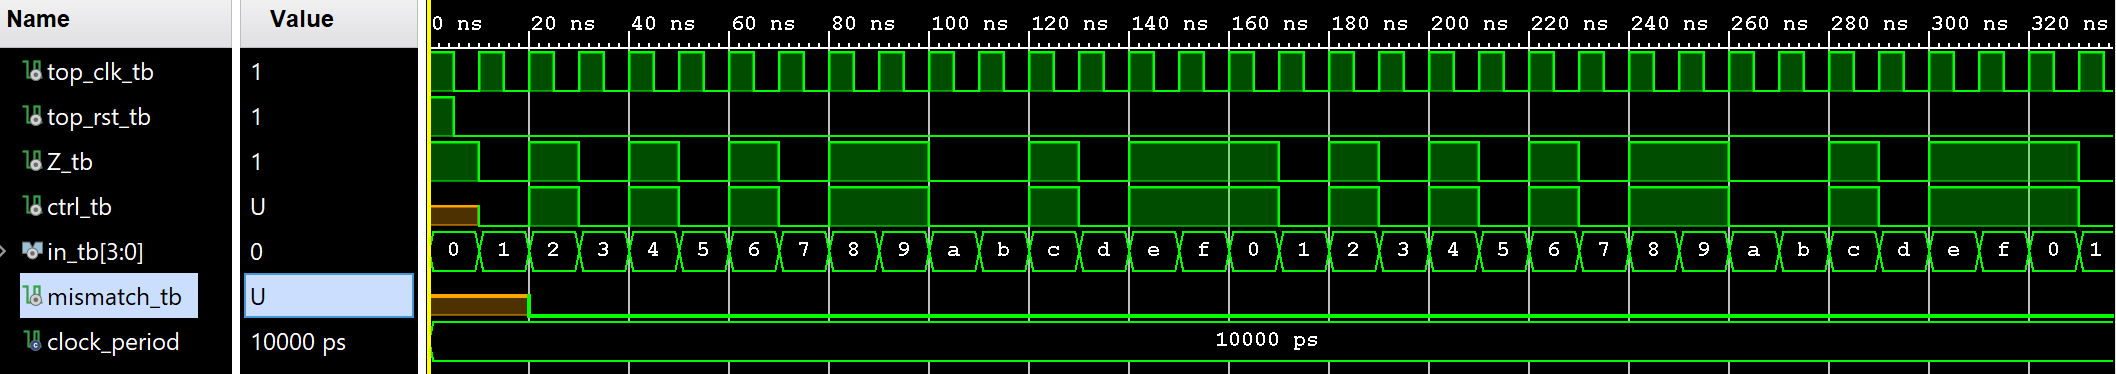
\includegraphics[width=\textwidth]{ECE4304_Midterm1_1_sim.png}
  \label{fig:1}
\end{figure}

\newpage

\section{2-bit Comparator}
\subsection*{Truth Table}
\begin{table}[H]
  \centering
  \begin{tabular}{cc:cc|ccc}
      \toprule
      $A_1$&$A_0$&$B_1$&$B_0$&$A>B$&$A=B$&$A<B$\\
      \midrule
      0&0 & 0&0 & 0&1&0\\
      0&0 & 0&1 & 0&0&1\\
      0&0 & 1&0 & 0&0&1\\
      0&0 & 1&1 & 0&0&1\\
      0&1 & 0&0 & 1&0&0\\
      0&1 & 0&1 & 0&1&0\\
      0&1 & 1&0 & 0&0&1\\
      0&1 & 1&1 & 0&0&1\\
      1&0 & 0&0 & 1&0&0\\
      1&0 & 0&1 & 1&0&0\\
      1&0 & 1&0 & 0&1&0\\
      1&0 & 1&1 & 0&0&1\\
      1&1 & 0&0 & 1&0&0\\
      1&1 & 0&1 & 1&0&0\\
      1&1 & 1&0 & 1&0&0\\
      1&1 & 1&1 & 0&1&0\\
      \bottomrule
  \end{tabular}
\end{table}

\newpage

\subsection*{Karnaugh Maps}
\begin{table}[H]
  \centering
  \begin{adjustbox}{width=\textwidth}
  \begin{tabular}{cc}
    \begin{karnaugh-map}[4][4][1][$B_1B_0$][$A_1A_0$]
      \minterms{4,8,9,12,13,14}
      \implicant{12}{9}
      \implicant{4}{12}
      \implicantedge{12}{12}{14}{14}
    \end{karnaugh-map}
    &
    \begin{karnaugh-map}[4][4][1][$B_1B_0$][$A_1A_0$]
      \minterms{0,5,10,15}
    \end{karnaugh-map}
    \\
    $(A>B)=\textcolor{red}{A_1\overbar{B_1}}+
    \textcolor{Green}{A_0\overbar{B_1}\overbar{B_0}}+
    \textcolor{YellowOrange}{A_1A_0\overbar{B_0}}$
    &
    $(A=B)=
    \overbar{A_1}\overbar{A_0}\overbar{B_1}\overbar{B_0}+
    \overbar{A_1}A_0\overbar{B_1}B_0+
    A_1\overbar{A_0}B_1\overbar{B_0}+
    A_1A_0B_1B_0
    $\\
    &$=(A_1\oplus B_1)(A_0\oplus B_0)
    $
    \\

    \quad\\ \\

    \begin{karnaugh-map}[4][4][1][$B_1B_0$][$A_1A_0$]
      \minterms{1,2,3,6,7,11}
      \implicant{3}{6}
      \implicant{1}{3}
      \implicantedge{3}{3}{11}{11}
    \end{karnaugh-map}
    &

    \\
    $(A<B)=\textcolor{red}{\overbar{A_1}B_0}
    +\textcolor{Green}{\overbar{A_1}\overbar{A_0}B_0}
    +\textcolor{YellowOrange}{\overbar{A_0}B_1B_0}
    $
    &
    \\
    $=\overbar{(A>B)+(A=B)}$
    \\
  \end{tabular}
\end{adjustbox}
\end{table}
\newpage
\subsection*{Code}
\subsubsection*{Comparator Circuit}
\lstinputlisting[style=VHDL]{ECE4304_Midterm1_VHDL/ECE4304_Midterm1_VHDL.srcs/sources_1/new/ECE4304_Midterm1_2.vhd}
\;\\
\subsubsection*{Testbench}
\lstinputlisting[style=VHDL]{ECE4304_Midterm1_VHDL/ECE4304_Midterm1_VHDL.srcs/sim_1/new/ECE4304_Midterm1_2_tb.vhd}
\;\\
\subsection*{Simulation Result}
As can be seen in figure \ref{fig:2}, all possible input combination was simulated and the circuit behave as expected with no mismatch found.
\begin{figure}[H]
  \centering
  \caption{Simulation Waveform of the Circuit}
  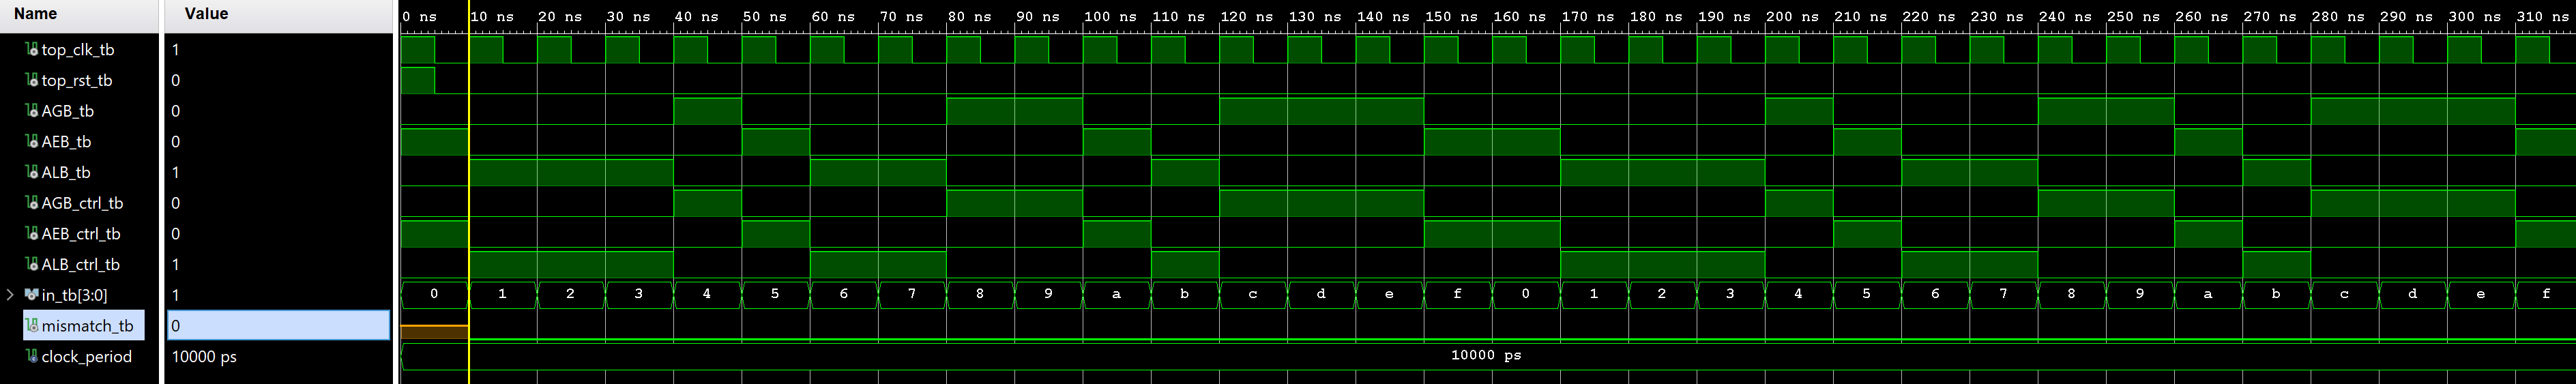
\includegraphics[width=\textwidth]{ECE4304_Midterm1_2_sim.png}
  \label{fig:2}
\end{figure}

\section{Clock Divider}

\subsection*{Code}
\subsubsection*{D Flip-flop}
\lstinputlisting[style=VHDL]{ECE4304_Midterm1_VHDL/ECE4304_Midterm1_VHDL.srcs/sources_1/new/DFlipflop.vhd}
\;\\
\subsubsection*{Clock Divider Circuit}
\lstinputlisting[style=VHDL]{ECE4304_Midterm1_VHDL/ECE4304_Midterm1_VHDL.srcs/sources_1/new/ECE4304_Midterm1_3.vhd}
\;\\
\subsubsection*{Testbench}
\lstinputlisting[style=VHDL]{ECE4304_Midterm1_VHDL/ECE4304_Midterm1_VHDL.srcs/sim_1/new/ECE4304_Midterm1_3_tb.vhd}
\;\\
\subsection*{Simulation Result}
As can be seen in figure \ref{fig:3}, the generated clock have a frequency of $f=\frac{1}{\SI{640}{\nano\second}}=\SI{1.5625}{\mega\hertz}\approx\SI{1.563}{\mega\hertz}$
\begin{figure}[H]
  \centering
  \caption{Simulation Waveform of the Circuit}
  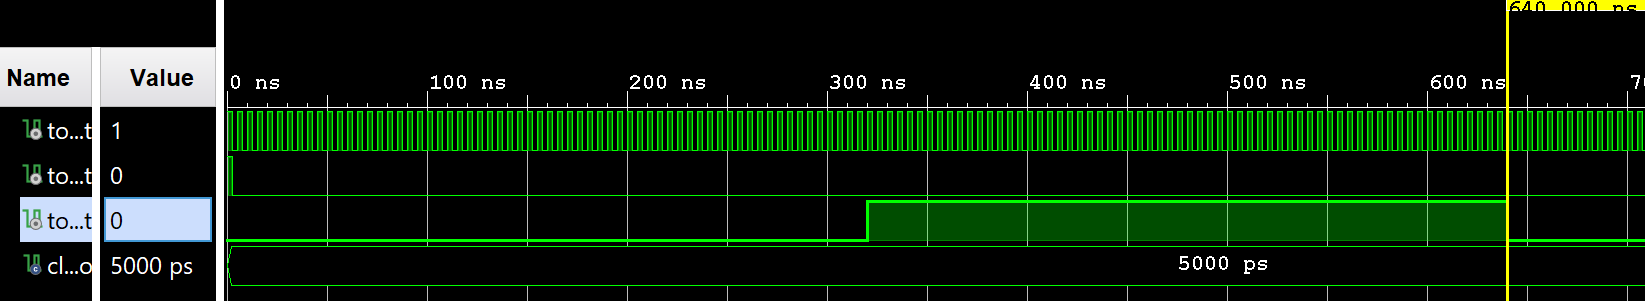
\includegraphics[width=\textwidth]{ECE4304_Midterm1_3_sim.png}
  \label{fig:3}
\end{figure}

\newpage

\section{Majority}


\section*{Truth Table}
\begin{table}[H]
  \centering
  \begin{tabular}{ccccc|c}
    \toprule
    $A$ & $B$ & $C$ & $D$ & $E$ & $maj$ \\
    \midrule
    0   & 0   & 0   & 0   & 0   & 0     \\
    0   & 0   & 0   & 0   & 1   & 0     \\
    0   & 0   & 0   & 1   & 0   & 0     \\
    0   & 0   & 0   & 1   & 1   & 0     \\
    0   & 0   & 1   & 0   & 0   & 0     \\
    0   & 0   & 1   & 0   & 1   & 0     \\
    0   & 0   & 1   & 1   & 0   & 0     \\
    0   & 0   & 1   & 1   & 1   & 1     \\
    0   & 1   & 0   & 0   & 0   & 0     \\
    0   & 1   & 0   & 0   & 1   & 0     \\
    0   & 1   & 0   & 1   & 0   & 0     \\
    0   & 1   & 0   & 1   & 1   & 1     \\
    0   & 1   & 1   & 0   & 0   & 0     \\
    0   & 1   & 1   & 0   & 1   & 1     \\
    0   & 1   & 1   & 1   & 0   & 1     \\
    0   & 1   & 1   & 1   & 1   & 1     \\
    1   & 0   & 0   & 0   & 0   & 0     \\
    1   & 0   & 0   & 0   & 1   & 0     \\
    1   & 0   & 0   & 1   & 0   & 0     \\
    1   & 0   & 0   & 1   & 1   & 1     \\
    1   & 0   & 1   & 0   & 0   & 0     \\
    1   & 0   & 1   & 0   & 1   & 1     \\
    1   & 0   & 1   & 1   & 0   & 1     \\
    1   & 0   & 1   & 1   & 1   & 1     \\
    1   & 1   & 0   & 0   & 0   & 0     \\
    1   & 1   & 0   & 0   & 1   & 1     \\
    1   & 1   & 0   & 1   & 0   & 1     \\
    1   & 1   & 0   & 1   & 1   & 1     \\
    1   & 1   & 1   & 0   & 0   & 1     \\
    1   & 1   & 1   & 0   & 1   & 1     \\
    1   & 1   & 1   & 1   & 0   & 1     \\
    1   & 1   & 1   & 1   & 1   & 1     \\
    \bottomrule
  \end{tabular}
\end{table}
\newpage
\section*{Karnaugh Maps}

\begin{karnaugh-map}[4][4][2][$DE$][$BC$][$A$]
\minterms{7,11,13,14,15,19,21,22,23,25,26,27,28,29,30,31}
\implicant{7}{15}[0,1]
\implicant{15}{11}[0,1]
\implicant{13}{15}[0,1]
\implicant{15}{14}[0,1]
\implicant{5}{15}[1]
\implicant{7}{14}[1]
\implicant{15}{10}[1]
\implicant{13}{11}[1]
\implicant{12}{14}[1]
\implicant{3}{11}[1]
\end{karnaugh-map}

\section*{function}
$$maj(A,B,C,D,E)=\textcolor{red}{CDE}+\textcolor{green}{BDE}+\textcolor{cyan}{BCD}+\textcolor{YellowOrange}{BCE}+\textcolor{blue}{ACE}+\textcolor{magenta}{ACD}
  +\textcolor{cyan}{ABE}+\textcolor{cyan}{ABD}+\textcolor{cyan}{ABC}+\textcolor{cyan}{ADE}$$

\newpage

\subsection*{Code}
\subsubsection*{Majority Circuit}
\lstinputlisting[style=VHDL]{ECE4304_Midterm1_VHDL/ECE4304_Midterm1_VHDL.srcs/sources_1/new/ECE4304_Midterm1_4.vhd}
\;\\
\subsubsection*{Testbench}
\lstinputlisting[style=VHDL]{ECE4304_Midterm1_VHDL/ECE4304_Midterm1_VHDL.srcs/sim_1/new/ECE4304_Midterm1_4_tb.vhd}
\;\\
\subsection*{Simulation Result}
As can be seen in figure \ref{fig:4}, all possible input combination was simulated and the circuit behave as expected with no mismatch found.
\begin{figure}[H]
  \centering
  \caption{Simulation Waveform of the Circuit}
  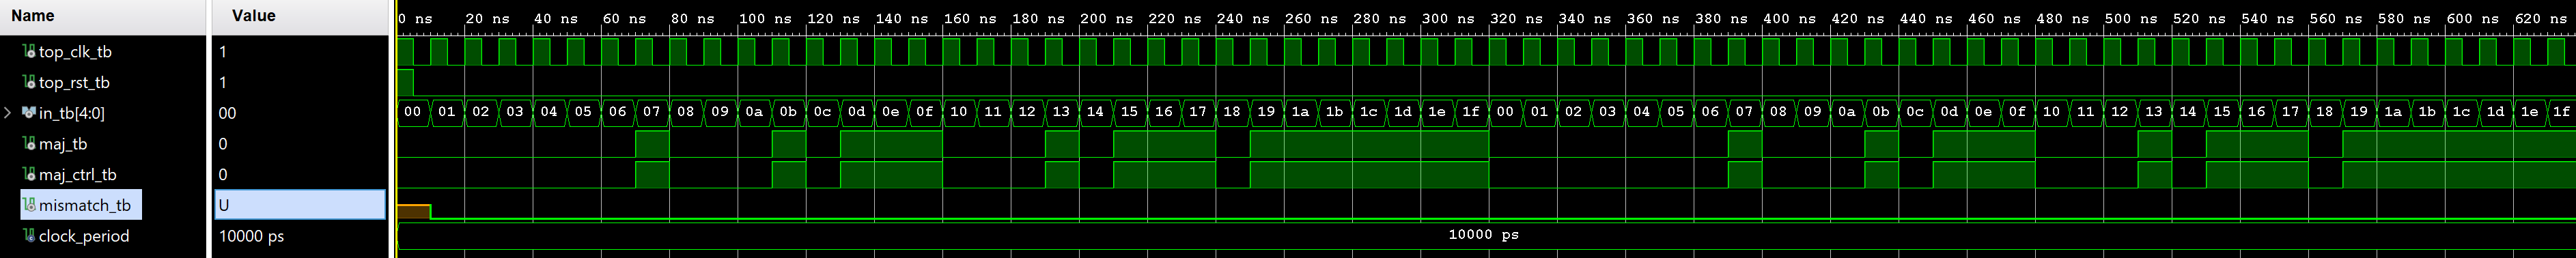
\includegraphics[width=\textwidth]{ECE4304_Midterm1_4_sim.png}
  \label{fig:4}
\end{figure}

\newpage

\section{N-bit Generic Multiplier}
\subsection{Theory}
Full Adder can be used to compose a multiplier as seen in \ref{fig:5_0}
\begin{figure}[H]
  \centering
  \caption{Sketch}
  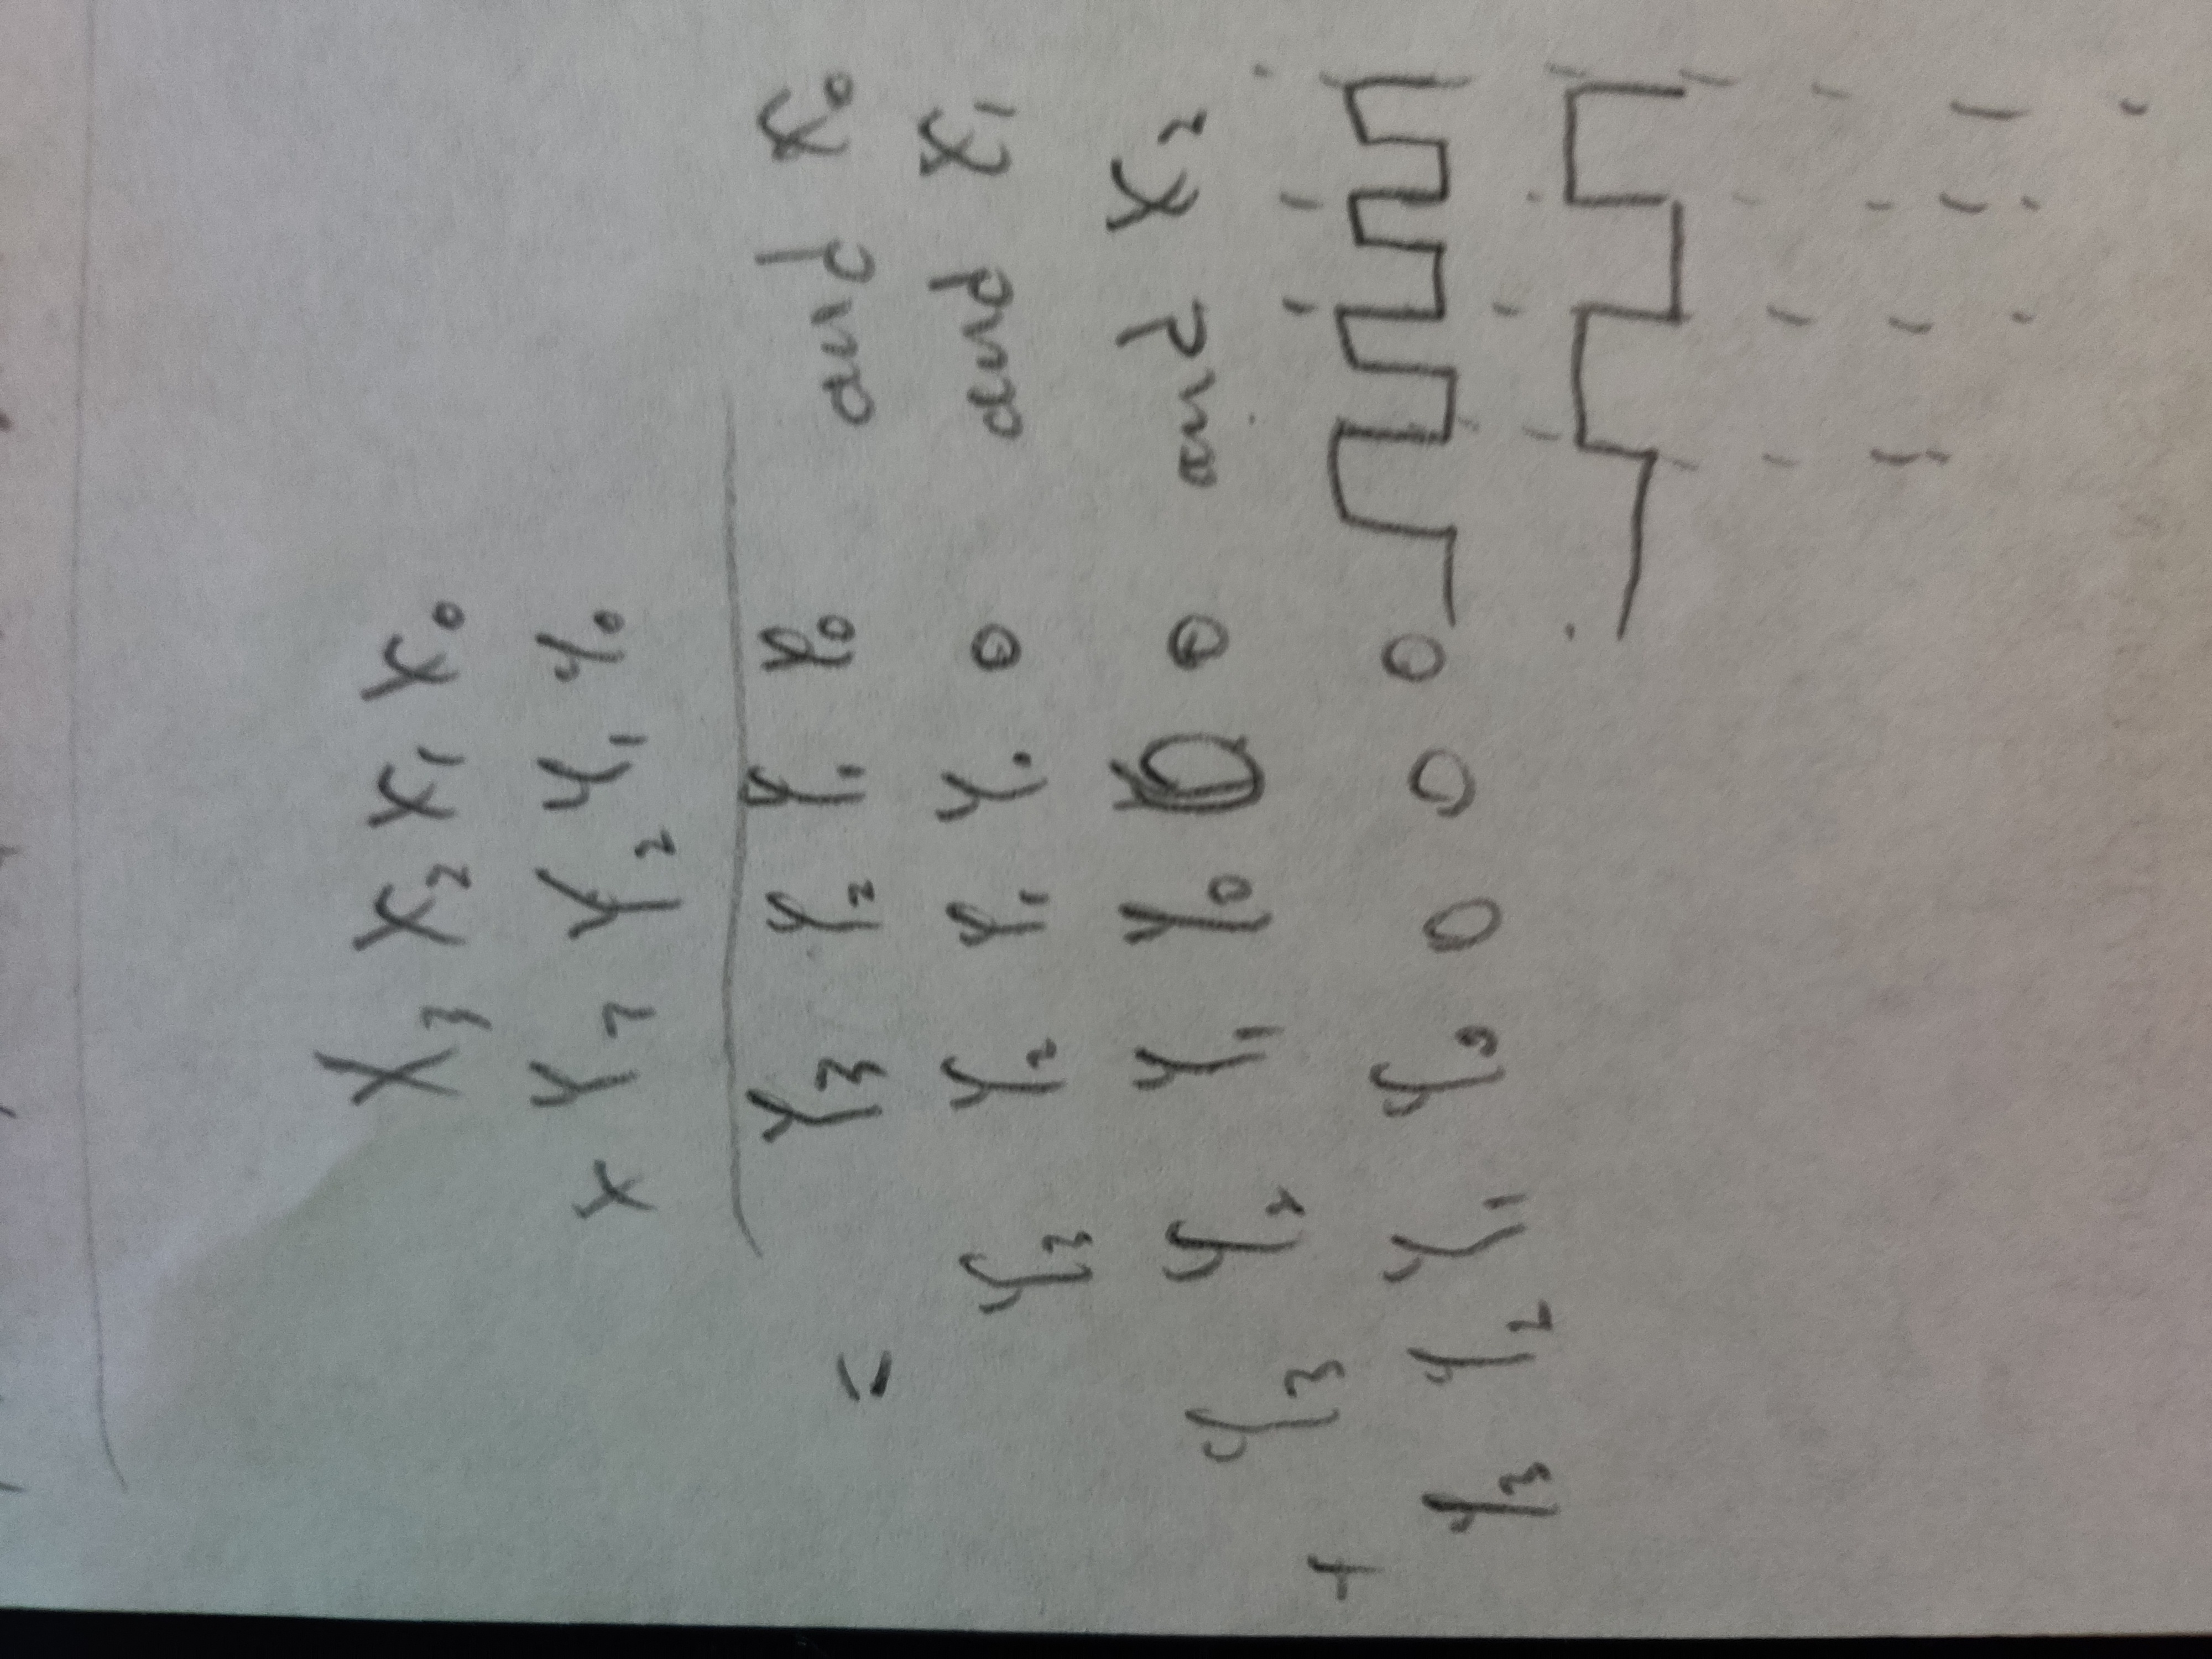
\includegraphics[width=\textwidth]{ECE4304_Midterm1_5_Sketch.jpg}
  \label{fig:5_0}
\end{figure}
\subsection*{Code}
\subsubsection*{N-bit Full Adder}
\lstinputlisting[style=VHDL]{ECE4304_Midterm1_VHDL/ECE4304_Midterm1_VHDL.srcs/sources_1/new/NFA.vhd}
\;\\
\subsubsection*{Majority Circuit}
\lstinputlisting[style=VHDL]{ECE4304_Midterm1_VHDL/ECE4304_Midterm1_VHDL.srcs/sources_1/new/ECE4304_Midterm1_5.vhd}
\;\\
\subsubsection*{Testbench}
\lstinputlisting[style=VHDL]{ECE4304_Midterm1_VHDL/ECE4304_Midterm1_VHDL.srcs/sim_1/new/ECE4304_Midterm1_5_tb.vhd}
\;\\
\subsection*{Simulation Result}
As can be seen in figure \ref{fig:5_1} and \ref{fig:5_2}, all possible input combination was simulated and the circuit behave as expected with no mismatch found.
\begin{figure}[H]
  \centering
  \caption{Simulation Waveform of the Circuit}
  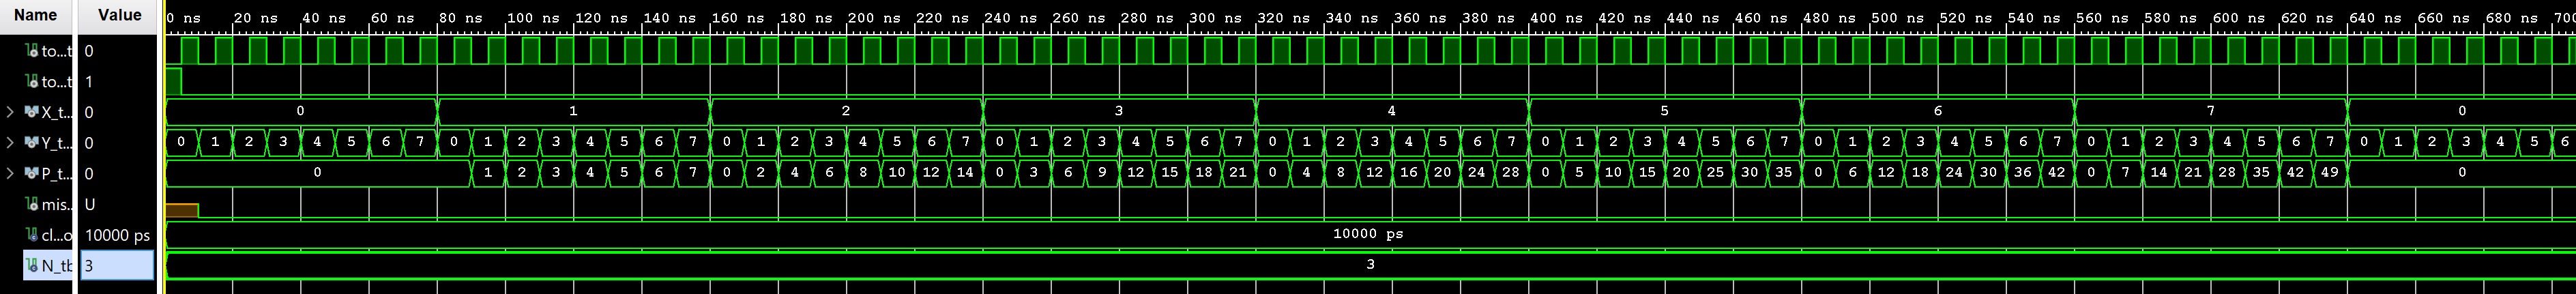
\includegraphics[width=\textwidth]{ECE4304_Midterm1_5_sim_1.png}
  \label{fig:5_1}
\end{figure}
\begin{figure}[H]
  \centering
  \caption{Simulation Waveform of the Circuit}
  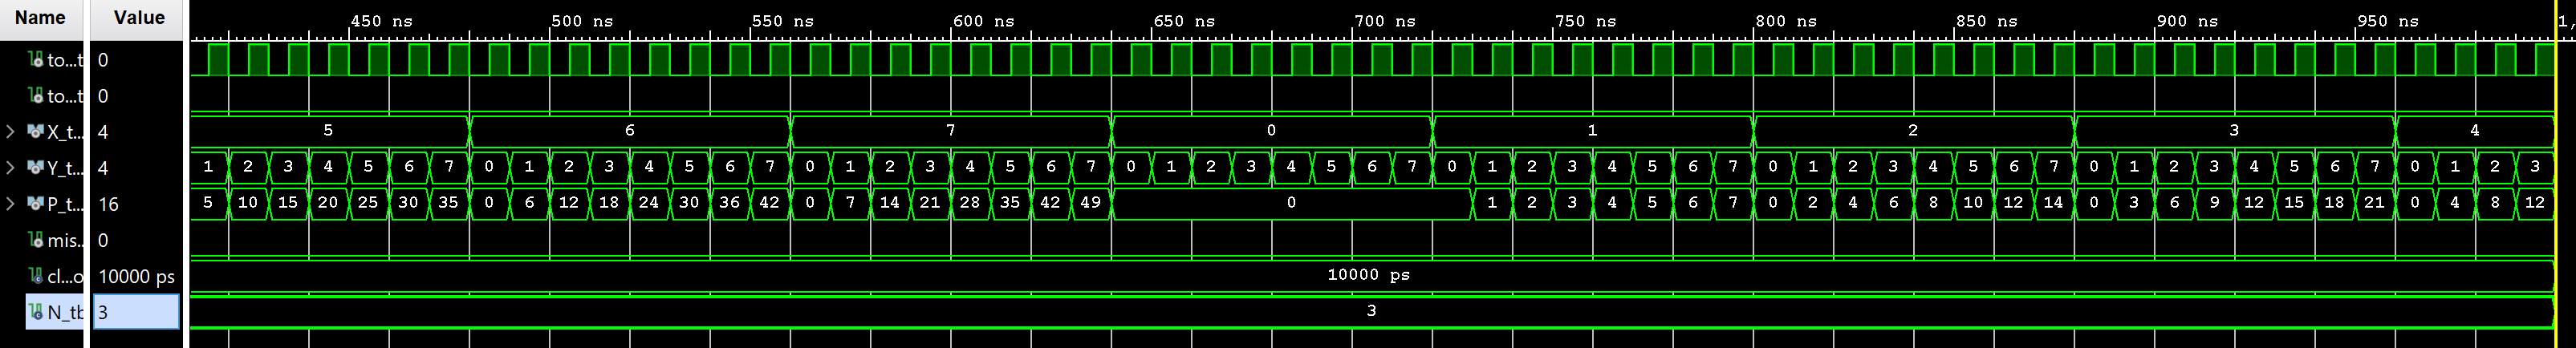
\includegraphics[width=\textwidth]{ECE4304_Midterm1_5_sim_2.png}
  \label{fig:5_2}
\end{figure}

\end{document}
